\chapter{Serverlose Softwarearchitektur}

Die Bereitstellung und der Betrieb von Software"=Applikationen sind zwei oft unterschätzte Kostenfaktoren. Viele technologische Entwicklungen der letzten Jahre, wie etwa Hardware"=Virtualisierung, Automatisierungswerkzeuge für Infrastruktur und Cloud"=Computing, haben diese Kosten bereits stark reduziert. Dennoch ist der Einsatz einer selbst verwalteten Infrastruktur aufwändig und erfordert intensive Zusammenarbeit zwischen Entwicklern, IT"=Administratoren und Release"=Managern.

Vor der Bereitstellung einer monolithischen Software steht zuerst die Dimensionierung und Beschaffung der benötigten Hardware"=Infrastruktur durch die IT-Abteilung. Diese muss danach noch an die Bedürfnisse und Voraussetzungen der Software angepasst werden. Die Installation der eigentlichen Software ist oft ein manueller oder halb"=automatisierter Prozess. Das ist langsam und fehleranfällig, aber meistens akzeptabel, denn eine monolithische Software hat lange Release"=Zyklen und besteht aus einem einzigen Artefakt. Erst das Microservice"=Architekturmuster hat eine isolierte, agile und effiziente Bereitstellung von Software vorangetrieben.

Mit \textit{Infrastructure-as-a-Service (IaaS)} bieten viele Cloud"=Computing"=Dienstleister die Möglichkeit, Server in wenigen Minuten bereitzustellen. Der Verwaltungsaufwand bleibt trotzdem relativ hoch, weil Betriebssystem"=Updates, IT"=Sicherheit, Netzwerkkonfiguration, \usw in der Verantwortung des Verwenders liegen. Viele Applikationen benötigen kaum Kontrolle über die Umgebung in der sie ausgeführt werden. Für diesen Fall ist die Verwendung eines \textit{Platform-as-a-Service (PaaS)} Dienstes meistens vorteilhafter. Hier übernimmt der \textit{PaaS}-Betreiber die vollständige Verwaltung der Hardware- und Betriebssystemebene. Der Dienstleistungsnehmer muss dafür nur seine Anwendung im richtigen Format bereitstellen, sowie die Kapazität und Skalierbarkeitseigenschaften festlegen.

Die Grundidee hinter \textit{Serverless Computing}, ist dem Softwareentwickler eine Plattform für die Bereitstellung von Diensten zu bieten, ohne dass sich dieser um Server, deren Konfiguration oder Kapazitätsmanagement kümmern muss. Bei \textit{IaaS} und \textit{PaaS} ist das nicht oder nur zum Teil gegeben.

Wie viele Konzepte im Microservice"=Umfeld lässt sich auch serverlose Softwarearchitektur nur schwer abgrenzen. Im nächsten Abschnitt werden die zwei zur Zeit häufigsten Ausprägungsformen näher betrachtet.

\section{Arten serverloser Softwarearchitektur}

Serverlose Softwarearchitektur ist ein sehr junges Konzept, dessen weitere Zukunft noch offen ist. Derzeit haben sich aber schon zwei unterschiedliche Sichtweisen auf dieses Themengebiet herauskristallisiert \cite{ServerlessArchitectures}.

In der älteren Sichtweise beschreibt der Begriff \textit{"`serverlos"'}, Applikationen die sehr stark auf vollständig verwaltete Dienste von Cloud"=Anbietern zurückgreifen. Darunter fallen beispielsweise verwaltete Datenbanken, Authentifizierungs- oder Benachrichtigungsdienste. Dieser Ansatz ersetzt also einen Großteil der Server"=Logikdurch Dienste von Drittanbietern. Daher hat sich auch die Bezeichnung \textit{Backend-as-a-Service} dafür etabliert. Ein Teil der Applikationslogik muss aber dadurch vom Client übernommen werden. Mit JavaScript und verschiedenen Bibliotheken für die Erstellung von Benutzeroberflächen, lassen sich die dafür benötigten \textit{Rich-Applications} effizient realisieren.

Seit etwa 2014 hat sich die Sichtweise durch die Einführung des Dienstes \textit{AWS Lambda} durch \textit{Amazon} etwas geändert. Dieser Dienst erlaubt es, einfache ereignisgesteuerte Funktionen zu schreiben, die in der Cloud in einer zustandslosen Ausführungsumgebung vollständig verwaltet laufen. Diese Funktionen enthalten fast ausschließlich Geschäftslogik und werden in Skript"=Dateien erstellt. Anstatt klobiger Artefakte können somit einfache Skript"=Dateien verteilt werden. Weil Funktionen das zentrale Bereitstellungsformat sind, ist dieser Ansatz unter dem Namen \textit{Functions-as-a-Service (FaaS)} bekannt. Der folgende Abschnitt beschäftigt sich intensiv mit dieser neuen Sichtweise auf serverlose Softwarearchitektur.

\section{Functions-as-a-Service}

Im Grunde erlaubt \textit{Functions-as-a-Service}, kleine Aufgaben in Form von Funktionen zu programmieren und skalierbar, ohne weiteren Aufwand in der Cloud zu betreiben. Der Entwickler kann sich voll auf die Geschäftslogik seiner Applikation konzentrieren und muss sich kaum noch um Infrastrukturaufgaben kümmern.

Wie in den allermeisten Programmiersprachen, sind Funktionen in diesem Kontext eine relativ kleine Quelltexteinheit, die Eingangs- in Ausgangswerte transformiert. Die Aktivierung erfolgt bei Programmiersprachen durch einen Funktionsaufruf. Hingegen bei \textit{FaaS}, durch das Auftreten bestimmter vom Entwickler festgelegter Ereignisse. Beispiele für derartige Ereignisse sind folgende:

\begin{itemize}
	\item Das Hinzufügen oder Manipulieren von Daten in einem Datenspeicher.
	\item Das Empfangen einer HTTP-Anfrage.
	\item Das Empfangen einer Nachricht von einem Nachrichtendienst.
	\item Das Auftreten eines zeitgesteuerten Ereignisses.
\end{itemize}

Eine Funktion ist nur dann sinnvoll, wenn sie auch Ausgaben oder zumindest Seiteneffekte produziert. In \textit{FaaS} können diese wieder sehr vielfältig sein. Meistens ist das Ergebnis, die Interaktion mit einem anderen Cloud"=Dienst wie \zB:

\begin{itemize}
	\item Das Hinzufügen oder Manipulieren von Daten in einem Datenspeicher.
	\item Das Senden einer HTTP-Antwort.
	\item Das Senden einer Nachricht an einen Nachrichtendienst.
	\item Das Versenden einer E-Mail.
\end{itemize}

Die folgenden Abschnitte beschreiben vielversprechende Anwendungsgebiete für \textit{FaaS}. Des Weiteren werden die Konzepte \textit{FaaS} und \textit{PaaS} voneinander abgegrenzt.

\subsection{Anwendungsgebiete}

Für \textit{FaaS} gibt es in den verschiedensten Bereichen sinnvolle Anwendungsgebiete. Hauptsächlich werden sie aber für kleine und abgeschlossene Funktionalitäten herangezogen. Beispielsweise eignet es sich sehr gut für die Konvertierung und Validierung von Daten. Eine Funktion kann auf ein bestimmtes Ereignis warten -- \zB dem Hinzufügen eines Elements in einer Warteschlange -- und danach die gewünschte Funktionalität ausführen. Das Ergebnis der Funktion kann \zB automatisch in eine Datenbank gespeichert oder an ein anderes System gesendet werden.

Microservice- und Cloud-Anwendungen verwenden oft eine große Anzahl an Cloud"=Komponenten, wie verschiedenen Datenspeicher, Warteschlangen und Nachrichtendienste. Damit alle Einzelkomponenten in Summe ein funktionstüchtiges Gesamtsystem bilden, ist viel Logik für die Verbindung und Administration der Komponenten notwendig. Im Englischen wird diese Art von Logik häufig als \textit{Glue-Code} bezeichnet, weil er die Einzelteile zum einem Ganzen "`zusammengeklebt"'. Die Interaktion mit Cloud"=Komponenten ist also ein essentielles Einsatzgebiet und ist deswegen ein großer Einflussfaktor auf das Programmiermodell von \textit{FaaS}.

Der Erfolg der Microservice"=Architektur und \textit{FaaS} führte bereits zur Entstehung eines möglicherweise neuen Paradigmas: \textit{Nanoservices} \cite{infoqFaaS}. Bei Microservices stehen einzelne Geschäftsanforderungen im Vordergrund. Mit Nanoservices werden einzelne Geschäftsanforderungen noch weiter auf Funktionsebene heruntergebrochen. Ein Beispiel für einen Microservice könnte ein Dienst für die Erstellung, Änderung und Nachverfolgung von Bestellungen in einem Online"=Shop sein. Mit Nanoservices wäre jede einzelne dieser Funktionen ein eigener Dienst.

\textit{Amazon} beschreibt in \cite{AwsMultiTier} wie klassische Drei"=Schicht"=Architektur, \zB Web- oder Mobile"=Anwendungen, mit serverlosen Technologie umgesetzt werden können. Darüber hinaus eignet sich \textit{FaaS} aber genau so gut für Microservice"=Architekturen. Die Einsatzgebiete sind daher sehr breit, was \textit{FaaS} zu einem mächtigen Werkzeug macht.

Viel Potential besteht in neuen Domänen, wie \textit{Internet of Things}, \textit{Chat-Bots} oder \textit{DevOps} \cite{NewStackAzurePreview}. In diesen Bereichen ist die Nachfrage nach kleinen, skalierbaren Programmen, die sich einfach entwickeln und betreiben lassen, sehr hoch. Durch die Einfachheit von \textit{FaaS} eignet es sich auch sehr gut für den Prototypenbau.

\subsection{Beziehung zu Platform-as-a-Service}

In vielen Bereichen überschneiden sich die Möglichkeiten von \textit{FaaS} mit denen anderer Technologien, wie \zB \textit{PaaS}. Dieser Umstand ist nicht weiter verwunderlich, da \textit{FaaS} auf der Basis von \textit{PaaS} aufbaut. Der signifikanteste Unterschied ist die ereignisgesteuerte Funktionsweise von \textit{FaaS}. Funktionen werden nach dem Auftreten eines bestimmten Ereignis nur für die Dauer einer Aktivierung ausgeführt. Daher bezahlt der Verwender auch nur die Anzahl der Aufrufe und die Dauer der Ausführungszeit. Bei \textit{PaaS} ist meistens zumindest eine ständig laufende virtuelle Maschine erforderlich, die auf Ereignisse wartet. Das verursacht Kosten, auch wenn die Maschine kaum oder gar nicht genutzt wird.

Skalierbarkeit ist in Cloud"-Computing ein essentieller Faktor. \textit{PaaS} bietet dafür die Möglichkeit, abhängig von Metriken wie Prozessorlast, die Anzahl der Instanzen auf denen die Anwendung ausgeführt wird, dynamisch zu erhöhen oder zu verringern. Dieser Ansatz erfordert bereits sehr wenig manuelles Eingreifen durch einen Entwickler oder Administrator. Aber \textit{FaaS} geht hier noch einen Schritt weiter und erfordert praktisch keine manuellen Handlungen, um die Funktion skalierbar zu machen. Es ist die Aufgabe des Cloud"=Anbieters, die Funktion automatisch zu skalieren. Weil die Funktionen zustandslos sind, kann man sie beliebig oft parallel ausführen.

Die Verwendung von \textit{PaaS} schränkt Technologieentscheidungen stark ein, weil man sich auf eine konkrete Plattform bindet. Bei \textit{FaaS} hingegen ist die Auswahl an möglichen Programmiersprachen sehr breit. Laufend fügen Cloud"=Anbieter neue Sprachen hinzu. Damit ist die Technologieabhängigkeit durch die Verwendung von \textit{FaaS} sehr viel geringer.

\subsection{Markt}

Alle namhaften Cloud"=Anbieter, wie Amazon, Microsoft, IBM und Google haben bereits \textit{FaaS}"=Produkte in ihrem Angebot. Die nachfolgenden Abschnitte zeigen die Funktionsweise und Prinzipien anhand von \textit{Microsoft Azure Functions}, da diese Implementierung unter der MIT-Lizenz Open-Source verfügbar ist und somit tiefe Einblicke in die Umsetzung bietet. 

\textit{Amazon AWS Lambda} ist von allen Produkten am längsten am Markt und bietet den größten Funktionsumfang. Jedoch haben auch die anderen Anbieter das Potential und die Nachfrage von \textit{FaaS} erkannt und versuchen seither, den Entwicklungsrückstand zu schließen.

Derzeit befindet sich dieses doch recht neue Thema noch stark im Wandel. Es ist sehr wahrscheinlich, dass sich einige Dinge in naher Zukunft verändern werden. Die Grundideen haben aber alle Anbieter ähnlich umgesetzt. Trotzdem unterscheiden sie sich in einzelnen Punkten:

\begin{itemize}
	\item Jeder Anbieter bietet unterschiedliche Programmiersprachen an. Es werden aber laufend neue Sprachen in die Produkte integriert.
	\item Auch wie das konkrete Skalierbarkeitsverhalten aussieht, muss beim jeweiligen Anbieter getestet werden.
	\item Meistens sind nur andere Dienste innerhalb des selben Cloud"=Anbieters mit \textit{FaaS} integriert. Dadurch kann sehr leicht eine starke Abhängigkeit zum gewählten Anbieter entstehen.
	\item Natürlich unterscheiden sich die einzelnen Angebote auch im Preis.
\end{itemize}

Derzeit investieren Cloud"=Anbieter sehr viel in die Entwicklung ihrer \textit{FaaS} Produkte. Das gibt einen Hinweis auf das große Potential dieser Technologie.

\section{Azure Functions}

Im März 2016 veröffentlichte die Firma \textit{Microsoft} eine Vorschauversion ihrer eigenen serverlosen Plattform mit dem Namen \textit{Azure Functions} \cite{AzFunIntro}. Nur ein halbes Jahr später folgte die erste offizielle Version \cite{AzFunGA}. \textit{Azure Functions} ist eine Erweiterung der ohnehin schon sehr umfangreichen \textit{Microsoft} Cloud"=Plattform. Diese Technologie eignet sich vor allem für die ereignisgesteuerte Verarbeitung und Transformation von Daten aus verschiedenen Datenquellen. Das deklarative Programmiermodell von \textit{Azure Functions} ermöglicht eine einfache Interaktion mit Daten- und Ereignisquellen. 

\textit{Microsoft} griff für die Implementierung von \textit{Azure Functions} auf folgende, schon länger in \textit{Microsoft Azure} enthaltene Dienste und Bibliotheken zurück \cite{AzFunJourney}:

\begin{itemize}
	\item \textit{App Service - Web App}
	\item \textit{App Service Plan}
	\item \textit{Site Control Manger (SCM)}
	\item \textit{Web Jobs}
	\item \textit{Web Jobs SDK}
\end{itemize}

Tatsächliche Neuentwicklungen waren folgende notwendig:

\begin{itemize}
	\item \textit{Web Jobs SDK Script}
	\item \textit{App Service - Function App}
	\item \textit{Dynamic Hosting Plan}
\end{itemize}

Die nachfolgenden Abschnitte geben einen Überblick hier aufgelisteten Bestandteile, die Entstehungsgeschichte und Anwendungsmöglichkeiten von \textit{Azure Functions}. Großteils beziehen sich die Grundlagen von \textit{App Services} und \textit{Web Jobs} auf \cite{AzWebEssentials4Devs}.

\subsection{Azure App Service}

\textit{App Service} ist in der \textit{Microsoft Azure} Cloud ein Oberbegriff für Services, die in die Kategorie \textit{Platform-as-a-Service} einzuordnen sind. Diese Services haben eine etwas konsequentere Interpretation von \textit{PaaS} als die älteren \textit{Cloud Services}. Bei einem \textit{App Service} übernimmt \textit{Microsoft} die Verwaltung der Infrastruktur, des Betriebssystems und der Laufzeitumgebungen. 

Ein \textit{App Service} ist einem sogenannten \textit{App Service Plan} zugeordnet. Dieser kann mehrere \textit{App Services} zusammenfassen, die auf einem oder mehreren Servern gemeinsam ausgeführt werden. Der \textit{App Service Plan} ist also eine abstrakte Infrastrukturbeschreibung, welche die Anzahl, Größe und das Skalierungsverhalten der virtuellen Maschinen festlegt. Daher wird er oft als \textit{Server Farm} bezeichnet.

Der nächste Abschnitt beschreibt mit \textit{Azure Web Apps} einen konkreten \textit{App Service}, der ein Grundbaustein hinter \textit{Azure Functions} ist.

\subsubsection{Azure Web App}

Eine \textit{Web App} ist in \textit{Microsoft Azure} der einfachste Weg um eine Web"=Anwendung bereitzustellen. Die virtuellen Maschinen des \textit{App Service Plan} in dem eine \textit{Web App} ausgeführt wird, sind bereits mit den gängigsten Webentwicklungsumgebungen ausgestattet. Damit lassen sich Web"=Anwendungen in unterschiedlichen Technologien gemeinsam betreiben. \textit{Web Apps} sind als eine Abstraktion eines Web"=Servers zu verstehen.

\subsection{Site Control Manager}

Die Funktionalität eines \textit{App Service} und somit auch einer \textit{Web App} ist mit Hilfe sogenannter \textit{Site Extensions} erweiterbar. Diese Erweiterungen werden im selben Kontext wie die eigentliche Web Anwendung ausgeführt. Der \textit{Site Control Manager} -- oft auch \textit{KUDU} genannt -- ist eine Erweiterung die bei jedem \textit{App Service} automatisch vorinstalliert ist. 

Anfänglich war die einzige Aufgabe des \textit{Site Control Manager} die Auslieferung des \textit{App Service} mittels Versionsverwaltungssystemen. Aber im Laufe der Zeit wurden weitere Funktionen ergänzt. Dazu zählt auch die Funktion \textit{Web Jobs}, welche die Abarbeitung von Hintergrundaufgaben ermöglicht. Für kleinere Aufgaben für die eine eigene virtuelle Maschine überdimensioniert wäre, sind \textit{Web Jobs} oft eine wirtschaftlichere Alternative.

\subsubsection{Web Jobs}

Als \textit{Web Job} eignen sich ausführbare Dateien oder unterstützte Skripte. Diese werden als eigener Prozess im Kontext eines \textit{App Service} entweder zeitgesteuert oder kontinuierlich ausgeführt. Damit können Hintergrundaufgaben überschüssige Kapazität ausnützen. Es kann aber auch zu negativen Effekten kommen, denn Hintergrundaufgaben können die Performanz der eigentlichen Web"=Anwendung für den Endbenutzer beeinflussen.

\subsection{Web Jobs SDK}

Die \textit{Web Jobs SDK} ist eine .NET"=Bibliothek für die Implementierung ereignisgesteuerter Hintergrundaufgaben. Das besondere daran ist das deklarative Programmiermodell, dass es erlaubt mit externen Datenquellen zu interagieren, ohne dafür extra Quelltext schreiben zu müssen \cite{WebJobsSdkBindingAttributes}.

Um vorab einen Einblick zu geben, zeigt Programm \ref{prog:webjobssdk} beispielhaft die Verwendung dieser Bibliothek. Der nächste Abschnitt enthält dann eine detailliertere Aufarbeitung der verwendeten Konzepte. Die folgende Aufzählung gibt eine Übersicht wichtiger Aspekte des Einführungsbeispiels:

\begin{itemize}
	\item Die Zeilen \textit{(1-5)} definieren eine Datenstruktur mit drei Attributen.
	\item Zeile \textit{(7)} startet die \textit{Web Jobs SDK} Laufzeitumgebung. Diese sucht per .NET Reflection nach kompatiblen Funktionen.
	\item Zeile \textit{(10)} definiert eine Funktion die ereignisgesteuert aufgerufen wird.
	\item Zeile \textit{(11)} definiert das Ereignis, das einen Funktionsaufruf auslöst. Hier wird die Funktion bei jedem neuen Eintrag in einer Warteschlangen aufgerufen und dessen Inhalt automatisch an den Funktionsparameter übergeben.
	\item Zeile \textit{(12)} definiert einen Ausgangsparameter. Wertzuweisungen an diesen Parameter werden automatisch in dem konfigurierten \textit{Blob Storage} gespeichert. Für den Pfad dieses Eintrags werden die aus dem Parameter in Zeile \textit{(11)} übergebenen Werte extrahiert.
	\item Zeile \textit{(13)} definiert einen weiteren Ausgangsparameter, der an eine andere Warteschlange weitergeleitet wird. Dieses Ereignis könnte wiederum einen anderen Funktionsaufruf auslösen. 
\end{itemize}

\begin{program}[!hbt]
\caption{Web Jobs SDK Beispiel}
\label{prog:webjobssdk}
\begin{CsCode}
  public class SensorData {
    public string SensorId { get; set; }
    public string Timestamp { get; set; }
    public double Value { get; set; }
  }
  class Program {
    static void Main() => new JobHost().RunAndBlock();
  }
  public class Functions {
    public static void ProcessSensorData(
      [QueueTrigger("sensorqueue")] SensorData sensorData,
      [Blob("values/{SensorId}/{Timestamp}")] out string sensorValue,
      [Queue("aggregationqueue")] out SensorData aggregationQueue) {
      sensorValue = sensorData.Value.ToString();
      aggregationQueue = sensorData;
    }
  }
\end{CsCode}
\end{program}

Obwohl die Funktion in Programm \ref{prog:webjobssdk} mit drei verschiedenen externen Datenquellen interagiert, enthält sie dafür fast keinen imperativen Quelltext, sondern lediglich eine deklarative Beschreibung in Form von Attributen. Die eigentliche Interaktion und das Warten auf Ereignisse ist die Aufgabe der \textit{Web Jobs SDK}. 

Eine \textit{Web Job} Anwendungen ist nichts anderes als eine gewöhnliche .NET Applikation mit einer Referenz auf die \textit{Web Jobs SDK}. Der nächste Abschnitt beschreibt wie statische Methoden einer \textit{Web Job} Anwendungen zu einem ereignisgesteuerten \textit{Web Job} werden.

Für viele Einsatzgebiete reicht dieses einfache, deklarative Programmiermodell aus. Es spricht aber nichts dagegen, die Interaktionslogik mit einer Datenquelle selbst im Funktionsrumpf zu implementieren. Das ist oft sogar notwendig, wenn der Funktionsumfang der deklarativen Variante nicht ausreicht. Der Grundgedanke ist jedoch derartigen repetitiven Standardquelltext durch deklarative Programmierung zu vermeiden.

\subsection{Bindungen}

Die zwei wesentlichen \textit{Web Job} Bindungen sind Trigger"=Bindungen und Nicht"=Trigger"=Bindungen. Erstere überwachen eine Ereignisquelle und lösen den Aufruf einer Job Funktion aus, wenn ein Ereignis auftritt. Zweitere binden Parameter einer Job Funktion an eine externe Datenquelle. Das kann sowohl zum Lesen, als auch zum Schreiben von Daten sein. Darum werden Nicht"=Trigger"=Bindungen in Eingangs- und Ausgangsbindungen eingeteilt. Jede Funktion muss genau eine Trigger"=Bindung haben, kann aber beliebig viele Nicht"=Trigger"=Bindungen enthalten.

Es gibt bereits eine Vielzahl vorhandener Bindungen. Entwickler können die Bibliothek aber auch mit selbst oder von Drittanbietern entwickelten Bindungen erweitern. Dazu muss man die wichtigsten dafür notwendigen Klassen kennen. Abbildung \ref{fig:webjobsclassdiag} zeigt den Bindungsmechanismus von Nicht"=Trigger"=Bindungen in einem stark vereinfachten Klassendiagramm.

\begin{figure}[!hbt]%
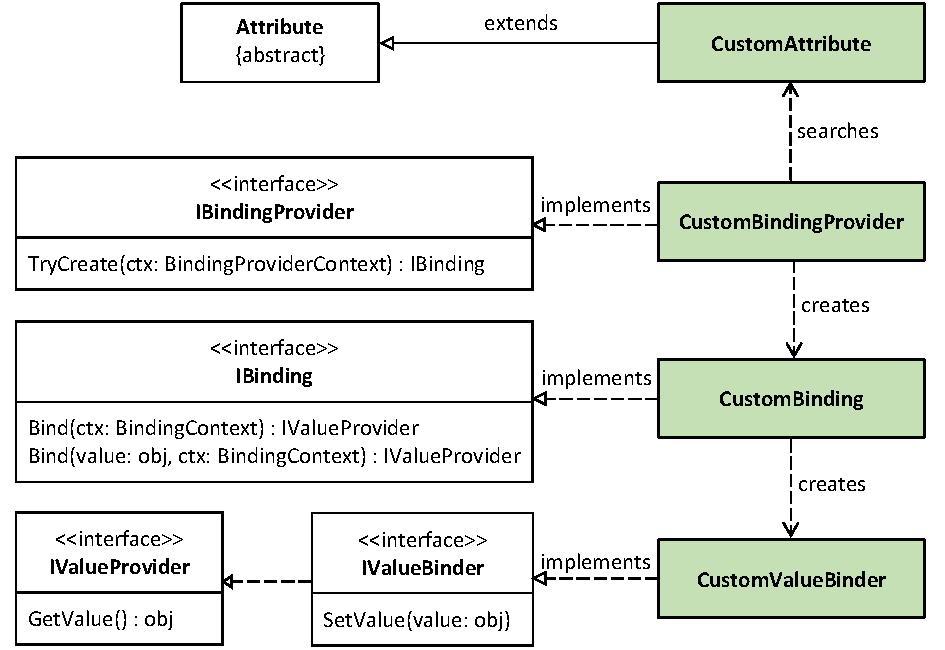
\includegraphics[width=\columnwidth]{webjob-ext-nontrigger-classdiag2}%
\caption{Web Jobs SDK Klassendiagramm (Nicht-Trigger-Bindung)}%
\label{fig:webjobsclassdiag}%
\end{figure}

Wie \cite{WebJobsSdkBindingProcess} beschreibt, ist der Bindungsprozess in zwei Phasen eingeteilt. Die nächsten Abschnitte beschreiben diese Phasen und geben somit auch Aufschluss darüber, wie die in Abbildung \ref{fig:webjobsclassdiag} skizzierten Klassen in Zusammenhang stehen.

\subsubsection{Startphase}

In der erste Phase beim Starten der Anwendung werden alle Funktionen auf ihre Tauglichkeit als \textit{Web Job} untersucht. Dieser Prozess umfasst folgende Schritte:

\begin{enumerate}
	\item Das Assembly der Anwendung wird nach allen Methoden in allen öffentlichen Klassen durchsucht.
	\item Für jeden Parameter einer Methode wird versucht eine Bindung zu erzeugen.
	\item Jeder registrierte \lstinline{I(Trigger)BindingProvider} bekommt die Möglichkeit eine Bindung über die Fabrikmethode \lstinline{TryCreate} zu erstellen. Diese Methode überprüft den Datentyp des Parameters und meistens die Existenz des Bindungs"=Attributs, welchess die Meta-Daten der Bindung beinhaltet. Sind die Voraussetzungen einer konkreten Bindung erfüllt, wird eine Bindung zurückgegeben.
	\item Wenn alle Parameter gebunden werden konnten, wird die Funktion im der \textit{Web Jobs} Laufzeitumgebung registriert.
	\item Für jede Trigger"=Binding wird zusätzlich die Überwachung der jeweiligen Ereignisquelle gestartet.
\end{enumerate}

\subsubsection{Laufzeitphase}

Nachdem alle Funktionen identifiziert wurden, beginnt die Laufzeitphase. In dieser Phase passiert die tatsächliche Bindung der Funktionsparameter. Dieser Ablauf lässt sich wie folgt zusammenfassen:
, wenn ein Funktionsaufruf durch ein Trigger"=Ereignis ausgelöst wurde.

\begin{enumerate}
	\item Ein Ereignis einer Trigger"=Bindung wird beobachtet und führt damit zur Ausführung der assoziierten Job Funktion.
	\item Für jeden gebundenen Parameter wird die \lstinline{BindAsync} Methode der zur Startphase festgelegten Bindung aufgerufen. In dieser passiert der eigentliche Interaktionsschritt mit einer externen Datenquelle, wie \zB dem Lesen von Daten aus einer Datenbank.
	\item Oft unterstützen Bindungen verschiedene Parametertypen, wie \zB \lstinline{String} oder \lstinline{Stream}. Die Bindung muss die tatsächlichen Werte auf den Datentyp der aufzurufenden Funktion konvertieren.
	\item Nachdem alle Parameter gebunden wurden, kann die eigentlich Funktion aufgerufen werden.
\end{enumerate}

\subsection{Web Jobs Script SDK}

Die \textit{Web Jobs Script SDK} ist das Herzstück von \textit{Azure Functions}. Es ist eine .NET Bibliothek, die eine interaktive Verwendung der sonst nur für .NET Applikationen geeigneten \textit{Web Jobs SDK} auch anderen Programmiersprachen zugänglich macht.

Die \textit{Web Jobs SDK} ist eine .NET Bibliothek und daher auch nur für .NET Anwendungen geeignet. Um die schon vorhandene Funktionalität auch für andere Sprachen und Platformen verfügbar zu machen, wurde die Bibliothek \textit{Web Jobs SDK Script} entwickelt.

- No Compilation step needed
- Simply change file - Runtime detects change
- Meta-Data in Attributes -> Meta-Data in Json file
- Adds the HTTP possiblity? (Script Host is running within the Functions Site extension)
- Folder structure - folder per function -> script files and config file
- No HTTP support needed -> run as continuous web job (otherwise sa a side extension)

\subsection{Azure Function App}

Part of app services
Evolution of web jobs
Many languages
Serverless
Groups belonging functions together

- In Azure waren viele Bausteine für eine serverlose Platform bereits vorhanden (Web Jobs, Web Jobs SDK, ...)


\subsection{Verrechnungsmodell}

- GB/s
- Vergleich mit lasttest und dedicated service plan

\subsection{REST-Schnittstellen implementieren}

- Einfach REST implementieren
- Generisch?

\subsection{Kaltstart}

\subsection{Erweiterbarkeit}

\subsection{Zusammenfassung}

Ereignisgesteruert, interation
vieles bereits möglich
erst jetzt wirklich serverless
wann serverless und wann dedicated
kaltstart verbesserungen
lego baukasten

\section{Evolution der Anwendungsentwicklung}

Dieser Abschnitt bezieht sich weitestgehend auf \cite{Cock16EvoFunc} und \cite{Cock17ShrinkingMS} in denen der Autor Adrian \citeauthor{Cock16EvoFunc} die Evolution von monolithischer Software"=Architektur hin zu Microservices und weiter zu ereignisgesteuerten serverlosen Anwendungen beschreibt. Außerdem werden die dafür verantwortlichen technischen und organisatorischen Entwicklungen identifiziert.

Software"=Applikationen haben die Aufgabe Geschäftswerte -- \textit{engl. business value} -- zu generieren. Dazu müssen sie den Benutzern die enthaltene Geschäftslogik zugänglich machen. Eine Funktion kann erst Geschäftswerte erzeugen, wenn sie dem Benutzer tatsächlich zur Verfügung steht. Daher sollte die Minimierung der Zeit zwischen der Erstellung der Geschäftslogik und der tatsächlichen Verfügbarkeit für den Endbenutzer für Unternehmen an oberster Stelle stehen. \citeauthor{Cock16EvoFunc} beschreibt diesen Zusammenhang in folgender Formel:

\begin{center}
\textit{time to value = creation cost + delivery cost}
\end{center}

In der Vergangenheit war die Dauer zwischen der Erstellung und der Auslieferung einer neuen Funktion oft sehr lange. Aufgrund des hohen Aufwands und der zahlreichen Risiken eines neuen Releases, wurden Anwendungen nur in sehr großen Zeitabständen ausgeliefert. Zu dieser Zeit waren monolithischen Anwendung, in Verbindung mit einer oder wenigen zentralen relationalen Datenbanken, der effizienteste Weg Geschäftslogik bereitzustellen. Software"=Design war zu einem großen Teil durch Performanzbedenken dominierten. Die folgenden drei Abschnitte erläutern wie Hardware-Fortschritte, Auslieferungsautomatisierung und organisatorische Veränderungen, diese Probleme verringerten und somit den Weg für Microservices und serverlose Anwendungen ebneten.

\subsection{Automatisierung der Softwareauslieferung}

Vor einigen Jahren war die Bereitstellung von Software noch ein manueller Prozess. Die Beschaffung, Installation, Konfiguration und Aktualisierung von physischen Servern war ein wesentlicher Zeit und Kostenfaktor. Durch diese langsamen Vorgänge wurden nur selten, dafür eine große Menge Geschäftslogik, in einer neuen Softwareversion ausgerollt.

Eine zusätzliche Herausforderung stellte die Kapazitätsplanung dar. Viele Server wurden aufgrund der langsamen Änderungszyklen  vorsichtshalber sehr großzügig dimensioniert. Das führte wiederum zu einer unökonomischen Ressourcenauslastung.

Die Automatisierung von Infrastrukturaufgaben regte ein Überarbeitung festgefahrener Softwareauslieferungsprozesse aus. Werkzeuge wie \textit{Chef} und \textit{Puppet} erlaubten es erstmals, Skripte für die automatische Provisionierung und Konfiguration von Infrastrukturkomponeneten zu erstellen. Zu diesen Komponenten zählen Server, Betriebssystem, Netzwerk, Konfiguration, aber auch die Applikationssoftware selbst. Heute bezeichnet man diese Möglichkeiten als \textit{Infrastructure-as-Code}, weil sich Infrastruktur mittels Quelltext erstellen und manipulieren lässt. \cite[135]{Httermann:2012:DD:2380958}.

Wenn sich Infrasturktur wie Quelltext behandeln lässt, ist es naheliegend, dass auch Softwareentwickler an diesem Prozess teilnehmen. Die Infrastrukturprovisionierung und -verwaltung verlagerte sich allmählich von den IT"= in die Softwareentwicklungsabteilungen. IT"=Abteilungen und Cloud"=Anbieter stellten den Entwicklern nur noch Programmierschnittstellen -- sogenannte APIs -- zur Verfügung, mit denen sie selbst die Infrastruktur nach ihren Bedürfnissen erzeugen und verändern konnten. Diese Zeit- und Kostenreduktion bei der Softwareauslieferung ermöglichten häufigere Releases und viel kleinere Anwendungen. Schlussendlich war das eine der Voraussetzung für die Microservice"=Architektur. Die Auslieferung von Service veränderte sich von einem langsamen und risikoreichen Prozess in einen automatisierten.

Alle Anbieter serverloser Plattformen haben auf die Erfahrungen der Vergangenheit aufgebaut und Automatisierbarkeit von Anfang an berücksichtigt. Softwaresystemen mit einer großen Anzahl von Funktionen wären manuell schwer handhabbar. 

\subsection{Leistungsverbesserung der Hardware}

Erst der technologische Fortschritt der Netzwerkübertragungs- und Festplattengeschwindigkeiten haben den Weg für echte Service"=orientierte Architekturen geebnet. Obwohl die Ideen hinter SOA schon lange existieren, wurden sie aufgrund von Performanzengpässen gar nicht oder nur unzureichend umgesetzt.

Nachrichten-orientierte Systeme bedeuten immer einen gewissen Mehraufwand für die Übertragung und Kodierung der Nachrichten. Die Netzwerkgeschwindigkeit hat sich in den letzten Jahren um das zehn- bis hundertfache gesteigert \cite{IEEEBandwidth}. In der Ethernet Spezifikation \textit{IEEE 802.3-2015} sind Übertragungsraten bis zu 100 Gigabit pro Sekunde spezifiziert.

Eine weitere Erschwernis die für Nachrichtenübertragung waren schwergewichtige, oft XML-basierte, Kodierungsprotokolle wie \zB SOAP. Erst die Entwicklung von leichtgewichtigeren \bzw effizienteren Protokollen, in Kombination mit den um Größenordnungen schnelleren Netzwerkverbindungen, leiteten den Siegeszug von Nachrichten-orientierten Systemen ein.

Auch in der Speichertechnologie passierte durch die Ablösung von magnetischen Festplatten durch \textit{Solid-State} Festplatten ein weiterer essentieller Technologiefortschritt. Magnetische Festplatten sind ihren neuen Konkurrenten vor allem bei zufälligen Lesezugriffen deutlich unterlegen. Diese schlechten Zugriffszeiten waren der Grund für das Design großer monolithischer Datenbanken. Geschäftslogikfunktionen mussten viele Operation in einer Transaktion durchführen, um die langsamen Zugriffszeiten zu kaschieren.

Auf der Basis der sehr schnellen \textit{Solid-State} Festplatten wurden eine Menge neuer \textit{NoSQL} Datenbanken entwickelt. Diese wiederum haben die Dezentralisierung und die in Abschnitt \ref{subsec:polyglot-persistance} beschriebene polyglotte Persistenz der bis dato hauptsächlich monolithischen Applikation vorangetrieben.

Auch Funktionen in \textit{FaaS} machen intensiven Gebrauch von Nachrichtenübertragung und verschiedenen Datenspeichern. Im Grunde transformieren sie Daten, wann immer sie über eine Nachricht oder andere Ereignisse benachrichtigt werden.

\subsection{Organisatorische Veränderungen}

Abschnitt \ref{sec:business-capabilities} hat bereits beschrieben, dass Microservices eine Umstrukturierung der Entwicklungsteams zur folge hatte. Projekt- oder Technologie"=bezogene Strukturen wurde in Produkt-bezogene transformiert. Sehr große Teams wurden in viele kleine Teams zerlegt, um den hohen Koordinationsaufwand zu reduzieren. Jedes der Teams ist für den gesamten Lebenszyklus eines oder mehrerer Dienste verantwortlich. Diese Struktur erlaubte eine viel agileren Entwicklung und erfordert weniger definierte Prozesse.

\subsection{Von Microservices zu serverlosen Anwendungen}

Wenn man Microservices auf die Spitze treibt, erfüllt jeder Service nur noch eine einzige Aufgabe. Aufgrund der großen Anzahl von Services in einer Microservice"=Architektur, erfordert dieser Ansatz eine extrem effiziente Bereitstellung von Services. Selbst automatisch erstellte virtuelle Server und Container sind dafür ungeeignet. Für diese Anforderung ist \textit{Function-as-a-Service} eine gute Wahl, denn Funktionen lassen sich in Bruchteilen einer Sekunde ausrollen.

Viele Services werden nur selten oder sehr unregelmäßig genutzt. In diesen Szenarien ist es schwierig mit Containern oder virtuellen Maschinen die Kapazität zum richtigen Zeitpunkt bereitzustellen. Die Auslastung der Ressourcen ist in solchen Fällen meistens nicht optimal. \textit{Function-as-a-Service} ist sehr gut für volatile Lastaufkommen geeignet. Anstatt Rechenkapazität dezidiert zu reservieren, werden Funktionen erst bei Bedarf ausgerollt.

Funktionen enthalten beinahe ausschließlich Geschäftslogik. Es ist kaum Standard- oder Plattform"=Quelltext notwendig. Damit gelingt es Entwicklern oft binnen weniger Tage Funktionen zu entwickeln. Dabei verbinden sie einfach eine Funktion mit anderen Funktionen oder anderen Drittanbieter"=Diensten. Ein großer Vorteil von \textit{Function-as-a-Service} ist, dass die entwickelten Funktionen automatisch hoch skalierbar und hoch verfügbar sind.

Alle zuvor beschriebenen Eigenschaften machen \textit{FaaS} zu einer wertvollen Ergänzung der Microservice"=Architektur. Es gibt aber durchaus Szenarien in denen es nicht gut geeignet ist, beispielsweise wenn die Last sehr groß und vorhersehbar ist.